\section{Jump Points}
In the previous section we developed simple rules for pruning neighbours during 
individual node expansions. We now extend this idea in order to define a 
macro-step operator which speeds up optimal search by selectively expanding
only certain nodes on a grid map. We term these nodes \emph{jump points}.
\par
The basic idea is straightforward: we give a simple example in Figure 
\ref{fig:jumppoints}(a).
Here we observe that when moving straight there are many cases where
the expanded node has only a single successor.
Since this successor cannot improve any other nodes on the open list we 
propose to evaluate it immediately, thereby avoiding an unnecessary list
maintenance operation. 
If we keep moving in the same direction we can continue this process until we 
either reach a node with more than one successor (a jump point), which we add to the open list instead of the nodes whose evaluation we expedited, or we find an 
obstacle which indicates that further search in this direction is fruitless.
\par
In the remainder of this section we will develop a macro-step operator which 
speeds up node expansion by identifying jump point successors in the case of
both straight and diagonal moves. We begin by making precise the concept of a
jump point:

\begin{definition}
\label{def:jump}
A node $x$ is designated a jump point if it satisfies at least one of the following
conditions:
\begin{enumerate}
\item{$x$ is the start or goal node.}
\item{$x$ is a node which, after pruning, is adjacent to at least one neighbour
whose evaluation is forced according to the rules in Section
\ref{sec:prunestraight} and Section \ref{sec:prunediagonal}.}
\item{$x$ has one or more successors which are themselves jump points.}
\end{enumerate}
\end{definition}

Note that we distinguish between a neighbour, which is immediately adjacent to
$x$ on the grid, and a successor which may not be. 
This is a fine but important distinction as in our work a neighbour can be a 
successor but the converse is not necessarily true.
Thus, when expand $x$, we will only consider its successors.


\subsection{Generating Successors}
The process by which we generate the set of successors necessary to expand a
node $x$ is given in Algorithm \ref{alg:successors}.
We start with the pruned set of neighbours immediately adjacent to $x$ (line 2).
Then, instead of immediately adding each neighbour $n$ to the set of successors
for $x$, we try to ``jump'' to a node that is further away but which lies in the 
same relative direction to $x$ as $n$ (lines 3:4). 
For example, if the edge $(x, n)$ constitutes a
straight move travelling \emph{right} from $x$, we look for a jump point among
the nodes immediately to the right of $x$.
If we find such a node, we add it to the set of successors instead of $n$.
In the case where we fail to find a jump point, we add nothing.
The process continues until the set of neighbours for $x$ is exhausted.

\input alg_jumpexpansion

\subsection{Jumping}
The process by which we identfy jump points is given in Algorithm
\ref{alg:jump}; it requires an initial node $x$, a direction of travel $dir$
(e.g. up, down, left right, etc) and the goal node $g$.
In rough overview, the algorithm attempts to establish whether $x$ has any 
jump point successors by stepping in the direction $dir$ and testing
if the node $n$ at that location satisfies the constraints outlined in 
Definition \ref{def:jump}.
When this is the case, $n$ is designated a jump point and returned (lines 5, 7
and 11).
When $n$ is not a jump node the algorithm recurses and steps again in direction
$dir$ but this time $n$ is the new initial node (line 12).
The recursion terminates when an obstacle is encountered and no further
steps can be taken (line 3).
Note that before each diagonal step the algorithm must first 
fail to detect any straight jump points (lines 9:11). 
This check corresponds to the third constraint of Definition \ref{def:jump} 
and is essential for preserving optimality.
We give an example of diagonal jump point identification in Figure
\ref{fig:jumppoints}(b).

\begin{figure}[tb]
       \begin{center}
		   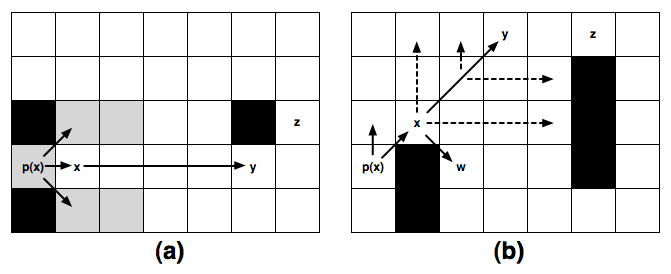
\includegraphics[scale=0.35, trim = 10mm 10mm 10mm 0mm]
			{diagrams/jumppoints.png}
       \end{center}
	\vspace{-3pt}
       \caption{Examples of straight (a) and diagonal (b) jump points.
Dashed lines indicate a sequence of interim node evaluations that reached
a dead end. Strong lines indicate eventual successor nodes.}
       \label{fig:jumppoints}
\end{figure}

\subsection{Optimality}
In this section we prove that for each optimal length path in a grid map there
exists an equivalent length path which can be found by only expanding jump
point nodes during search (Theorem \ref{theorem:jumping}).  Our result is
derived by identifying for each optimal path a symmetric alternative which we
split into contiguous segments. We then prove that each \emph{turning point}
along this path is also a jump point.

\begin{definition}
\label{def:turningpoint}
A \emph{turning point} is any node $n_{i}$ along a path where the direction of
travel from the previous node $n_{i-1}$ to $n_{i}$ is different to the direction
of travel from $n_{i}$ to the subsequent node $n_{i+1}$.
\end{definition}

Before proving our main result, we will first derive an interim result that
in which we show jumping from one jump point node to any other is optimal.

\begin{theorem}
\label{theorem:jumping}
For each optimal length path between two jump point nodes on a grid there exists
an equivalent length path that mentions only jump point nodes.
\end{theorem}
\begin{proof}
Let $\pi$ be an arbitrarily chosen optimal path between two jump point nodes
on a grid.  
%We will show that for each $\pi$ there exists a symmetric path $\pi'$ which has
%the same length and mentions only nodes that are jump points.
\par
First, we re-order $\pi$ s.t. diagonal moves appearing along the path are taken
as early as possible. This is a simple operation performed on pairs of adjacent
edges appearing along $\pi$ where $(i, j)$ is a straight edge and $(j, k)$ is a
diagonal edge.
The objective is to replace each such pair of edges with two new edges: 
$(i, j')$, which is a diagonal move and $(j', k)$ which is a straight move. 
The operation is successful if:
\begin{itemize}
\item $(i, j'$) and $(j', k)$ are both valid moves; i.e. node $j'$ is not an
obstacle.
\item $(i, j') + (j', k) = (i, j) + (j + k)$; i.e. the cost of
the path $\pi$ is unchanged by the operation.
\end{itemize}
We apply this procedure repeatedly until no further re-ordering of the moves
is possible and return $\pi'$, a new optimal path which is symmetric
to the original.
\par
Next, we divide $\pi'$ into a series of adjacent segments s.t. 
$\pi' = \pi'_{0} + \pi'_{1} + \ldots + \pi'_{n} $. Each $\pi'_{i} = \lbrace n_{0}, n_{1},
\ldots, n_{k-1}, n_{k} \rbrace$ is a subpath along which all moves involve
travelling in the same direction (e.g.  only ``up'' or ``down'' etc).  Notice
that with the exception of the start and goal, every node at the beginning and
end of a segment is also a turning point.
\par
Since each $\pi'_{i}$ consists only of moves in a single direction
(straight or diagonal) we can use Algorithm \ref{alg:jump} to jump from $n_{0}
\in \pi'_{i}$, the node at beginning of each segment to $n_{k} \in \pi'_{i}$, the
node at the end, without necessarily stopping to expand every node in between.
Intermediate expansions may occur but the fact that we reach $n_{k}$
optimally from $n_{0}$ is guaranteed.
It remains to show only that both $n_{0}$ and $n_{k}$ are identified as
jump points and thus necessarily expanded. 
By Corollary \ref{lemma:turningpoints} each turning point is 
also a jump point, so every turning point node must be expanded during search.
Only the start and goal remain. These are jump points by definition and must
also be expanded.
\end{proof}

\begin{corollary}
\label{lemma:turningpoints}
Each turning point of $\pi'$ is also a jump point.
\end{corollary}
\begin{proof}
Let $n_{k}$ be an arbitrary turning point node along $\pi'$. 
%First, we observe that exactly of the edges $(n_{k-1}, n_{k})$ or $(n_{k}, n_{k+1})$ 
%must involve a diagonal step (Corollary \ref{corollary:diagonalturn}).
There are two cases to consider, depending on whether $n_{k}$ is next
to an obstacle or not.
\par
In the first case, the obstacle must be blocking of the four cardinal 
moves (``up'', ``down'', ``left'' or ``right''); otherwise we can re-write 
$\pi'$ s.t. $n_{k}$ is no longer mentioned.
If one of the four cardinal moves is blocked, $n_{k}$ has at least one
forced neighbour. This satisfies the second condition in Definition
\ref{def:jump} and we conclude $n_{k}$ is a jump point.
\par
In the second case $n_{k}$ is not adjacent to any obstacle but the edge
from its predecessor $n_{k-1}$ must be a diagonal step; otherwise we can 
re-write $\pi'$ s.t. $n_{k}$ is no longer mentioned.
Since $n_{k}$ is not adjacent to an obstacle, the next turning point along 
$\pi'$ must be; otherwise we can once more re-write $\pi'$ s.t $n_{k}$ is no longer
mentioned. Further, the next turning point along $\pi'$ must be reachable 
by a series of straight moves; otherwise $\pi'$ is not optimal.
This is sufficient to satisfy the third condition in Definition \ref{def:jump} and
we conclude $n_{k}$ is a jump point.
\end{proof}

%\begin{theorem}
%\label{theorem:jumpoptimal}
%Searching with jump points is optimal.
%\end{theorem}
%\begin{proof}
%Let $s$ and $g$ be arbitrarily chosen locations on a grid that represent
%and goal location associated with a particular pathfinding query.
%By definition $s$ is a jump point. Since it has no parent 
%allowable direction away from $s$ computing all possible jump point successors.
%By Lemma \ref{lemma:jumping} we can travel optimally from the
%successors of $s$ to any other jump point on the grid.
%Since the goal $g$ is a jump point by definition, it follows that an optimal
%length path from $s$ to $g$ is returned.
%\end{proof}
%
